\chapter{Signal Reflection}
    \section{Định nghĩa Phản xạ tín hiệu (Signal Reflection)}
    \section{Hệ số phản xạ (Reflection Coefficient)}
        \begin{figure}[h]
            \centering
            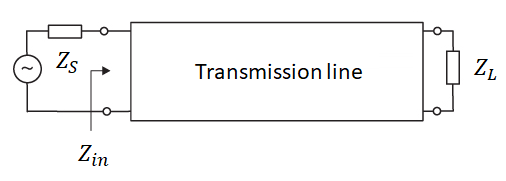
\includegraphics[width=0.5\textwidth]{figures/transmission_line.png}
            \caption{Transmission line schematic with input, source, and load impedances.}
        \end{figure}
        Hệ số phản xạ $\Gamma$\cite{cadence2023sparams}\cite{cadence2021transmission} biểu thị \textbf{mức độ sóng phản xạ lại} khi đi qua một giao diện có sự \textbf{không phù hợp trở kháng}\par
        
        \subsection{Hệ số phản xạ tại đầu tải}
            $$\Gamma_L = \frac{Z_{L} - Z_0}{Z_{L} + Z_0}$$
            \begin{itemize}
                \item $Z_{L}$: Trở kháng của tải (Load impedance)
                \item $Z_0$: Trở kháng đặc trưng của đường truyền
                \item $|\Gamma|$: Hệ số phản xạ, nằm trong khoảng $\left[0,1\right]$, giá trị càng lớn thì phản xạ càng cao
            \end{itemize}
        
        \subsection{Hệ số phản xạ tại nguồn}
            Phản xạ tại nguồn khi tín hiệu quay ngược về phía đầu vào của đường truyền:
            $$\Gamma_S = \frac{Z_{in} - Z_S}{Z_{in} + Z_S}$$
            \begin{itemize}
                \item $Z_{in}$: Trở kháng đầu vào của đường truyền
                \item $Z_S$: Trở kháng của nguồn
            \end{itemize}
